\documentclass[12pt]{article}
\usepackage[a4paper, total={6.5in, 8in}]{geometry}
\usepackage[T1]{fontenc}
\renewcommand{\familydefault}{\sfdefault}
\renewcommand{\baselinestretch}{1.5}
\usepackage[dvipsnames]{xcolor}

\usepackage[english]{babel}
\usepackage[utf8]{inputenc}
\usepackage{amsmath}
\usepackage[super, comma]{natbib} 
\usepackage{graphicx}
\usepackage{enumitem}
\usepackage{listings}
\usepackage[font={small,it},labelfont=bf,tableposition=top,justification=centering]{caption}
\usepackage{array}
\usepackage{textcomp}
\usepackage{tabularx}
\usepackage{threeparttable}
\usepackage{float}
\usepackage{epstopdf}
\epstopdfsetup{update}
\usepackage{xcolor}
\usepackage{mdframed}

%----------------------------------------------------------------------------
% text commands
%----------------------------------------------------------------------------
\newcommand{\addref}{\textbf{[addref]}}
\newcommand{\comment}[1]{[{\textbf{#1}}]}
\newcommand{\ie}{i.e.\ }
\newcommand{\eg}{e.g.\ }
\newcommand{\etal}{{\em et al.}\ }

\newcommand{\AMBER}{\textsc{Amber}}
\newcommand{\CHARMM}{\textsc{Charmm}}
\newcommand{\DLPOLY}{\textsc{Dl-Poly}}
\newcommand{\GROMACS}{\textsc{Gromacs}}
\newcommand{\LAMMPS}{\textsc{Lammps}}
\newcommand{\NAMD}{\textsc{Namd}}

%============================================
\setitemize{noitemsep,topsep=0pt,parsep=0pt,partopsep=0pt}
\definecolor{light-gray}{gray}{0.9}
\definecolor{beaublue}{rgb}{0.74, 0.83, 0.9}


\lstset{basicstyle=\ttfamily\small,
  backgroundcolor=\color{light-gray},
  breaklines=true,
  xleftmargin=\parindent,
  xrightmargin=\parindent,
  literate={~} {$\sim$}{1}
  }


\begin{document}

\begin{titlepage}
 \centering \vspace*{3cm}
 \textbf{\Huge ForConX} \\ \vspace{1cm}
 \textbf{\Large A Force Field Conversion Tool Based on XML} \\ \vspace{2cm}
 \begin{figure}[H]
  \centering
  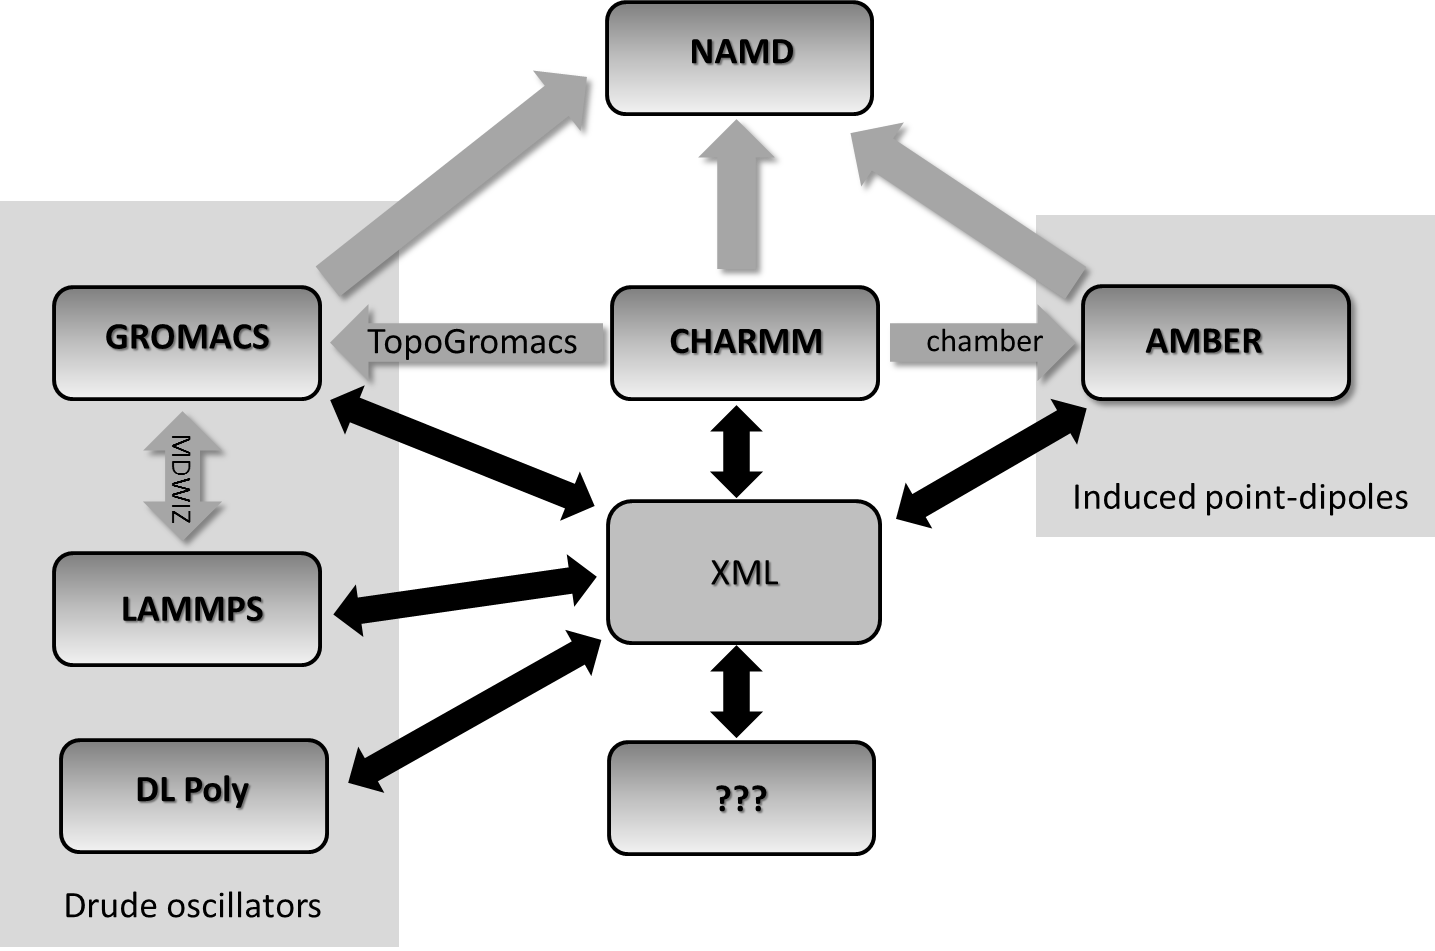
\includegraphics[width=0.8\textwidth]{ForConX_bw.png}
 \end{figure}
 \textbf{\large Version 0.1}\\

\end{titlepage}

\tableofcontents
\pagebreak

 
%%%%%%%%%%%%%%%%%%%%%%%%%%%%%%%%%%%%%%%%%%%%%%%%%%%%%%%%%%%%%%%%%%%%%%%%%%%%%%%%%%%%%%%%%%%%%%%%%%%%%%%%%%%%%%%%%%%%%%%%%%%%%%%%%%%%%%%%%%%%%%%%%%%%%%%%%%%%%%%%%%%%%%%%%%%%%
\section{Introduction}
\textsc{ForConX} is a Python code for conversion between force field files of
different Molecular Dynamics (MD) simulation packages. Currently, the following MD programs
are available:
\begin{itemize}
\item \AMBER
\item \CHARMM
\item \DLPOLY
\item \GROMACS
\item \LAMMPS
\end{itemize}
but can easily be extended to new MD program by writing an interface to the central
XML document. ForConX is free software, distributed under the terms of the GNU General Public License version 3, 
as published by the Free Software Foundation and included in the source code documentation. 
This program is distributed in the hope that it will be useful, but WITHOUT ANY WARRANTY, without even the implied warranty of 
MERCHANTABILITY or FITNESS FOR A PARTICULAR PURPOSE. See the GNU General Public License for more details.  
In no event the authors will be liable to you for damages, including any general, special, incidental or consequential damages 
(including but not limited arising out of the use or inability to use the program, to loss of data or data being rendered inaccurate, 
or losses sustained by you or third parties, or a failure of the program to operate with any other programs),
even if the author has been advised of the possibility of such damages.

The features of \textsc{ForConX} are described in the following publication
\begin{mdframed}[backgroundcolor=gray!40]
\textit{``ForConX - A Forcefield Conversion Tool Based on XML``}\\
V. Lesch, D. Diddens, C.E.S. Bernardes, B. Golub, A. Dequidt, V. Zeindlhofer, \\
M. Sega, C. Schr\"oder, \textit{J. Comp. Chem.} \textbf{2017}, 38, 629.
\end{mdframed}
Please cite if you are using this tool.
\clearpage{}

\subsection{The central idea}
\textsc{ForConX} consists of three phases as visible in Fig.~\ref{fig_phases}.
In the first phase the force field files of a MD program is translated to a XML document. The XML document is checked during the second phase. The last phase concerns
the conversion from the XML document to the force field files of target MD program.
\begin{figure}[bh]
  \centering
  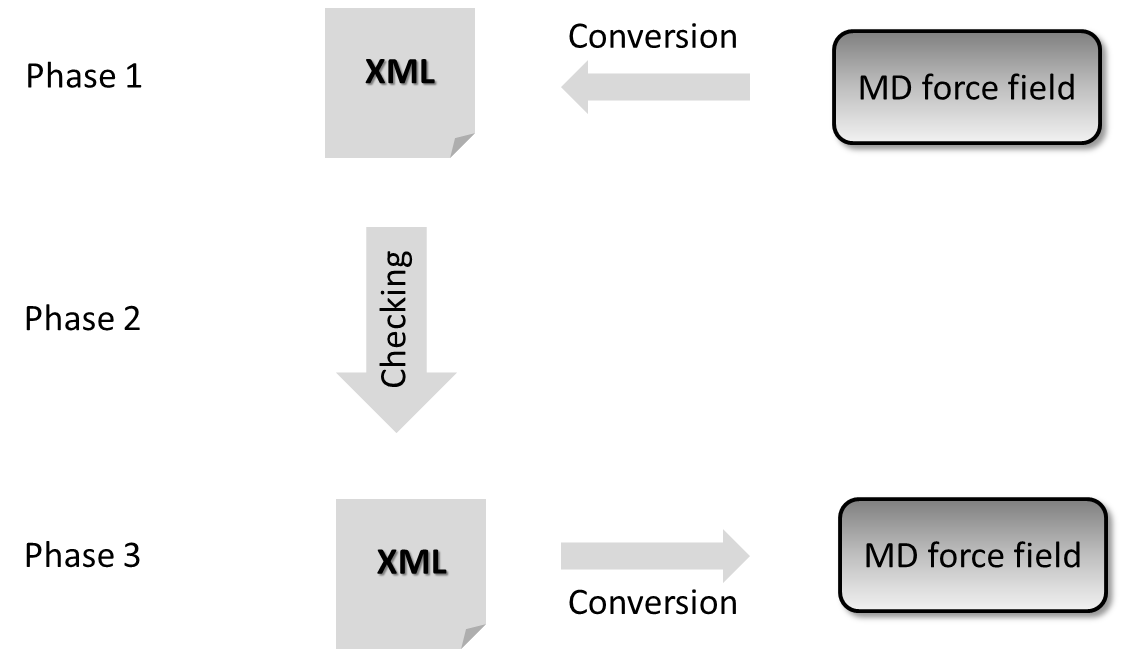
\includegraphics[width=10cm]{./ForConX_ablauf.png}
   \caption{The ForConX conversion process.}
   \label{fig_phases}
\end{figure}

The conversion of a force field from one MD program to another may necessitate several runs of \textsc{ForConX}. During the first run, the XML document is augmented
by the information \textsc{ForConX} gained from the original MD force field files. If the program terminates because of insufficient information, the user may 
add, remove or modify particular lines in the XML document and re-run starting at Phase 2 and consequently not from the original MD program but from the XML 
information. In any case, Phase 2 is always part of a \textsc{ForConX} run. Here, all XML lines are checked for completeness and if the information in the 
parameter section fits to that defined for the molecules given in the topology section.

Making a new MD program available in \textsc{ForConX} is realized by writing an interface from that MD program to the XML structure and back in the other direction.
As a result, it is not necessary to write pairwise conversion tools between the MD programs.

%%%%%%%%%%%%%%%%%%%%%%%%%%%%%%%%%%%%%%%%%%%%%%%%%%%%%%%%%%%%%%%%%%%%%%%%%%%%%%%%%%%%%%%%%%%%%%%%%%%%%%%%%%%%%%%%%%%%%%%%%%%%%%%%%%%%%%%%%%%%%%%%%%%%%%%%%%%%%%%%%%%%%%%%%%%%%
\section{Installation and running}
To install ForConX, Python 2.x must be present in the operating system. 

\subsection{Installation}
Please unzip the source code in a directory and change to the ForConX directory. In principle, the file setup.py should be present in that directory.
The program can be compiled using the standard python method:

\begin{lstlisting}
 $ python setup.py install --user
\end{lstlisting}
This will place the executable (in principle) in the standard directories
\begin{lstlisting}
 .local/bin
\end{lstlisting}
or 
\begin{lstlisting}
 ~/Library/Python/X.X/bin
\end{lstlisting}
in case of MacOs.
Now, you should be able to execute \textsc{ForConX} at any directory on your system.


\subsection{Running}

To run the program, type:
\begin{lstlisting}
$ forconx inputfile.xml
\end{lstlisting}
where \texttt{inputfile.xml} is a XML file containing the information 
regarding the input files to be converted and the output files format (see details below).


%%%%%%%%%%%%%%%%%%%%%%%%%%%%%%%%%%%%%%%%%%%%%%%%%%%%%%%%%%%%%%%%%%%%%%%%%%%%%%%%%%%%%%%%%%%%%%%%%%%%%%%%%%%%%%%%%%%%%%%%%%%%%%%%%%%%%%%%%%%%%%%%%%%%%%%%%%%%%%%%%%%%%%%%%%%%%
\section{XML file}
The XML input file can be composed by several elements that are included in a <ForConX> ... </ForConX> section.  
For any run, the xml file must contain an <input>, <output> and <molecule> (one for each molecule) elements.  
\begin{lstlisting}[basicstyle=\linespread{1.1}\ttfamily]
<?xml version="1.0" ?>
<ForConX>
    <input md="MD program 1">
    ...
    </input>

    <output md="MD program 2">
    ...
    </output>

    <molecule name="MOLNAME1" nmol="..."/>
    ...
</ForConX>
\end{lstlisting}
The remaining sections are facultative and include the details of the bonded and nonbonded force field parametrizations, 
that will be filled when this information is retrieved from the initial input files.

Currently, the MD programs {\AMBER}, {\CHARMM}, {\DLPOLY}, {\GROMACS} and {\LAMMPS}  are supported. Alternatively,
one may start from the XML structure. During the conversion process, \textsc{ForConX} writes after the completion 
of each phase a XML document: forconx\_1.xml, forconx\_2.xml and forconx\_3.xml.
These files can be used to add information and re-run \textsc{ForConX}.

\clearpage{}
\subsection{$<$input$> \ldots <$/input$>$ or $<$output$> \ldots <$/output$>$}
This XML section concerns the original MD program and has the same keywords as $<$output$> \ldots <$/output$>$ except 
for the citation defined in $<$reference$> \ldots <$/reference$>$:
\begin{lstlisting}[basicstyle=\linespread{1.1}\ttfamily]
<input md="XML">
   <energy   unit="KCAL"      />
   <distance unit="ANGSTROEM" />
   <coordinates pdb="..." />
   <reference>
    <title> ... </title>
    <author> ... </author>
    <journal> ... </journal>
    <volume> ... </volume>
    <year> ... </year>
    <pages> ... </pages>
   </reference>
   ...
 </input>
\end{lstlisting}
Energy, distance and polarizability unit are usually defined by the MD program. For example, {\CHARMM} explicitly
uses kcal/mol, {\AA} and {\AA$^3$}. Consequently, if md=''CHARMM`` \textsc{ForConX} automatically overwrites
the unit definitions with the default values mentioned above.
Other programs allow for several units, \textit{e.g.} {\DLPOLY} may use kcal/mol, kJ/mol or even K as energy unit.
Also when starting from a XML structure, the units has to be specified with the option tabled in Tab.~\ref{tab:input2}.
During the conversion process, the unit definitions of $<$input$> \ldots <$/input$>$ and $<$output$> \ldots <$/output$>$    
are used to convert the force field parameters into the units typical for the target MD program.

The force field file structure differs for each MD program. Sometimes several files are needed to setup a
force field. MD program specific parts are given in Tab.~\ref{tab:input1}.

\begin{table}[H]
 \newcommand{\rowsep}{2mm}
 \def\arraystretch{0.8}
 \caption{Units used in the input/output sections.}
 \label{tab:input2}
  \begin{threeparttable}
  \begin{tabularx}{\textwidth}{p{6cm}p{3.5cm}l}
  \hline
  \textbf{Element}	&	\textbf{Key}	& Unit\\ \hline
<energy unit="KEY"/>	&	KCAL	 & kcal/mol\\
                        &       KJ       & kJ/mol = 0.239 kcal/mol\\
                        &       K        & Kelvin\\
<distance unit="KEY"/>	&	ANGSTROEM & \AA	\\
		        &	NM	  & nm = 10 \AA \\
<polarizability unit="KEY"/>	& ANGSTROEM & \AA$^3$ \\
				&	NM  & nm$^3$ = 1000 \AA$^3$ \\  
				&  BOHR     & $a_0^3$ = (0.529 \AA)$^3$ \\
				\hline
  \end{tabularx}
  \end{threeparttable}
\end{table}
\begin{table}[H]
 \newcommand{\rowsep}{2mm}
 \def\arraystretch{0.8}
 
 \caption{List of elements that can be used in the input and 
	  output sections for the different MD simulation programs supported by ForConX.}
 \label{tab:input1}
  \begin{threeparttable}
  \begin{tabularx}{\textwidth}{p{5cm}l}
  \hline
  \textbf{MD Program}	&\textbf{Element}	\\   \hline
  AMBER			& <lib file="FILE.lib"/> \\
			&<frcmod file="amber\textunderscore new.frcmod"/> \\ [\rowsep]
  CHARMM		&<topology  file="FILE.rtf"/>\\
			&<parameter file="FILE.prm"/>\\
			&<crd       file="FILE.crd"/>\\[\rowsep]
  DLPOLY		&<field     file="FIELD"/>	\\
                        &<config    file="CONFIG" />\\[\rowsep]
  GROMACS		&<top       file="FILE.top"/>	\\[\rowsep]
  LAMMPS\tnote{a}	&<command   file="input.lmp"/>\\
			&<data      file="data.lmp"/>\\
			&<pair      file="pair\textunderscore coeffs.lmp"/>\\
			&<molecule  ext=".mol"/>	\\[\rowsep]
			\hline
  \end{tabularx}
  \begin{tablenotes}
   \footnotesize
   \item[a] only the element “command” is required to read the original LAMMPS input files
  \end{tablenotes}
  \end{threeparttable}
\end{table}


\subsection{$<$molecule$> \ldots <$/molecule$>$}
To perform a MD program 1 $\rightarrow$ XML $\rightarrow$ MD program conversion, it is necessary to indicate each 
molecule to be converted as:
\begin{lstlisting}
<molecule name="MOLNAME" nmol="..."/>
\end{lstlisting}
where “MOLNAME” is the name of the molecular specie in the input files 
to for conversion, followed by the number of molecules, “nmol”, in the configuration file.
It is possible to define several molecules
\begin{lstlisting}
<molecule name="MOLNAME1" nmol="..."/>
<molecule name="MOLNAME2" nmol="..."/>
\end{lstlisting}
Here, the atom names within a particular molecule has to be unique but maybe the very same in different molecules.

After phase 1 of conversion, \textsc{ForConX} augments the XML file which now looks like this:
\begin{lstlisting}[basicstyle=\linespread{1.1}\ttfamily\small]
<molecule name="..." nmol="...">
    <atom name="..." type="..." mass="..." charge="..." 
	  alpha="..." />
    <virtual name="..." type="..." charge="..."  
	     zmatrix="... ... ..." r="..." 
	     theta="..." phi="..." />
    <bond name="... ..." />
    ...
    <angle name="... ..." />
    ...
    <dihedral name="... ... ... ..." />
    ...
    <improper name="... ... ... ..." central="..." />
    ...
</molecule>
\end{lstlisting}
All atoms have a unique name, an atom type, a mass and a partial charge. The polarizability alpha is optional.
Virtual atoms possess no mass but can be defined using a z-matrix style. $r$ is the distance between the virtual
atom and the first atom in zmatrix. $theta$ is the angle between the virtual atom and the first and second atom
in zmatrix and $phi$ the dihedral angle between the virtual atom and all atoms defined in zmatrix.
All bonds between atoms are defined by <bond> with alphabetically sorted atomnames.
This bond information is very important since the autogeneration of angle and dihedrals rely on a complete
definition of all bonds within a molecule. Furthermore, during the check of the XML structure, dihedral 
and impropers are only accepted, if all corresponding bonds are present. 

Only bonds, angles, dihedrals and improper torsions defined in the <molecule>-section are taken into 
account for the conversion, even if additional potentials in the <bonds>,<angles>, <dihedrals>
and <impropers> section exists.

\subsection{$<$bonds$> \ldots <$/bonds$>$}
This section contains all force field parameters of harmonic bonds and Morse potentials. They are
stored in the XML structure in the following way:
\begin{lstlisting}[basicstyle=\linespread{1.1}\ttfamily\small]
<bonds>
    <harm type="... ..." r0="..." k="..." />
    <mors type="... ..." r0="..." D0="..." beta="..." />
</bonds>
\end{lstlisting}
In contrast to the bonds in <molecule>, the identifier is the atom type.
Harmonic bonds and Morse potentials cannot be defined for the very same type=''... ...``.

\subsection{$<$angles$> \ldots <$/angles$>$}
\textsc{ForConX} knows harmonic angles and Urey-Bradley potentials.
\begin{lstlisting}[basicstyle=\linespread{1.1}\ttfamily\small]
<angles>
    <harm type="... ... ..." k="..." theta0="..." />
    <urey type="... ... ..." k="..." r0="..." />
</angles>
\end{lstlisting}
Since Urey-Bradley potentials are used to introduce anharmonicity to harmonic angles,
the type is not an unique identifier in this section.

\subsection{$<$dihedrals$> \ldots <$/dihedrals$>$}
Cosine torsion and Ryckaert-Bellemans potentials can be handled by \textsc{ForConX}.
\begin{lstlisting}[basicstyle=\linespread{1.1}\ttfamily\small]
<dihedrals>
    <cos  type="... ... ... ..." n="... ... ..."
	  delta="... ... ..." k="... ... ..." />
    <ryck type="... ... ... ..." k="... ... ... ... ... ..."/>
</dihedrals>
\end{lstlisting}
However, the type is unique and hence these potential are mutual exclusive.

\subsection{$<$impropers$> \ldots <$/impropers$>$}


\begin{lstlisting}[basicstyle=\linespread{1.1}\ttfamily\small]
<impropers>
    <cos delta="... ... ..." k="... ... ..." n="... ... ..." 
	  type="... ... ... ..."/>
    <ryck type="... ... ... ..." k="... ... ... ... ... ..."/>
    <harm type="... ... ... ..." k="..." theta0="..."	/>  
</impropers>
\end{lstlisting}


\subsection{$<$nonbonded$> \ldots <$/nonbonded$>$}

\begin{lstlisting}[basicstyle=\linespread{1.1}\ttfamily\small]
<nonbonded>
    <mixing_rules epsilon="geometric" sigma="arithmetic"/>
    <atom type="... ..." epsilon="..." sigma="..."  
          vdw14="..." elec14="..." />
      ...
    <vdw type="... ..." epsilon="..." sigma="..."  
         vdw14="..." elec14="..." />
      ...
</nonbonded>
\end{lstlisting}


%%%%%%%%%%%%%%%%%%%%%%%%%%%%%%%%%%%%%%%%%%%%%%%%%%%%%%%%%%%%%%%%%%%%%%%%%%%%%%%%%%%%%%%%%%%%%%%%%%%%%%%%%%%%%%%%%%%%%%%%%%%%%%%%%%%%%%%%%%%%%%%%%%%%%%%%%%%%%%%%%%%%%%%%%%%%%
\clearpage{}
\section{Developers guide}
\textsc{ForConX} is written in Python 2. 
An overview of all \textsc{ForConX} code files and where to find them is given in Fig.~\ref{fig:classes}.
The ./potentials directory contains python files for the energy potentials used. All core routines of \textsc{ForConX} are stored in the ./md\_xml directory and 
should not be changed.
In addition to these directories, each MD program has its own directory, \textit{e.g.} ./charmm. 
\begin{figure}[bh]
\centering
 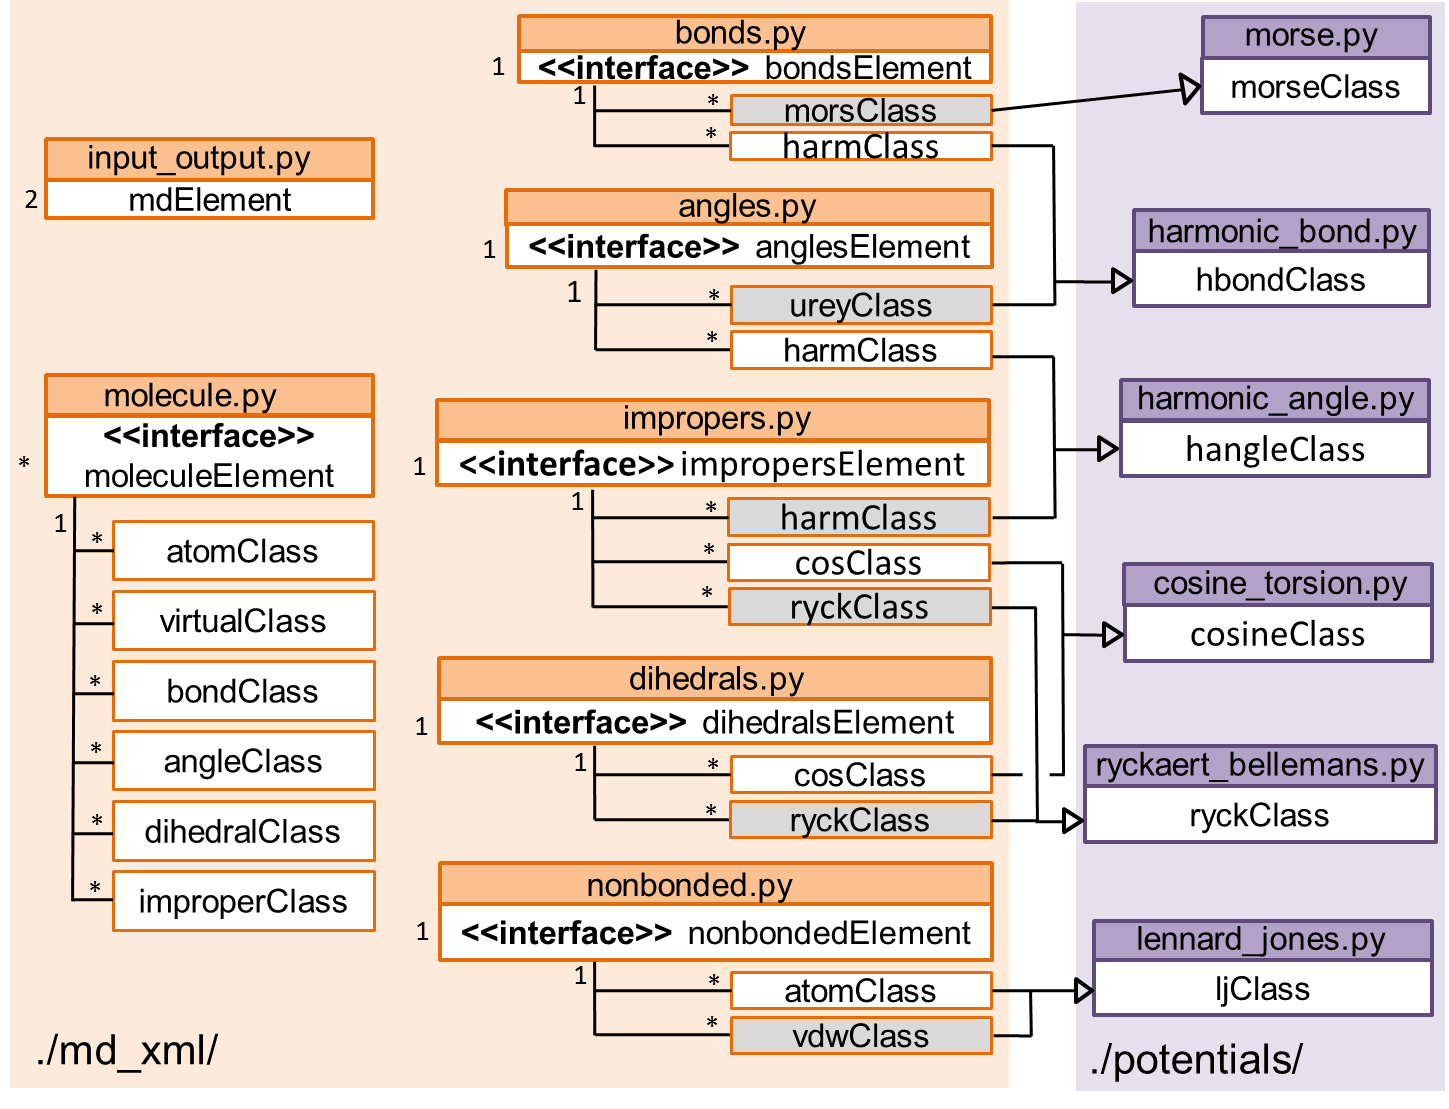
\includegraphics[width=\linewidth]{ForConX_Classes.png}
 \caption{Python classes in \textsc{ForConX} and where to find them.}
 \label{fig:classes}
\end{figure}

\subsection{./md\_xml}
The core routines of \textsc{ForConX} are in this directory:
\begin{itemize}
 \item input\_output.py
 \item molecule.py
 \item bonds.py
 \item angles.py
 \item dihedrals.py
 \item impropers.py
 \item nonbonded.py
\end{itemize}
Each of these files is responsible for a particular segment of the XML document which can be deduced from their names. Except input\_output.py, these Python files
contain and $\ll$interface$\gg$ to all classes which are also defined in the same Python file. 
Some of these classes have a parent class defined in ./potentials.

\subsection{./potentials}
This directory contains Python files for each energy potential used in \textsc{ForConX}. 
Overloading ensures that not only a value of a particular property can be set but also that the XML structure is immediately updated.

\subsection{MD program}
Each MD program has its own directory which contain at least three files:
md2xml.py and xml2md.py for the force field conversion and xyz.py for the production of a coordinate file on a basis of a temporary forconx.pdb. Consequently,
xyz.py is able to convert the MD specific coordinate file to a PDB file and vice versa. md2xml.py and xml2md.py convert the force field files using the Python objects
described in the next section.

\subsection{XML structure}
\textsc{ForConX} uses the xml module of Python which is documented at 
\begin{lstlisting}[basicstyle=\linespread{1}\ttfamily\small]
https://docs.python.org/2/library/xml.etree.elementtree.html
\end{lstlisting}

{\noindent}root is a pointer to the XML tree. The present molecules  can then be find 
\begin{lstlisting}[basicstyle=\linespread{1}\ttfamily\small]
import xml.etree.ElementTree as ET
import sys

xmlfile = sys.argv[1]
root =  ET.parse(xmlfile).getroot()
for mol in root.findall('molecule'):
  molname = mol.get('name')
\end{lstlisting}

\subsection{Elements and Classes}
In order to gain access to all properties of the atom and virtual atoms of that molecule, molecule.py offers moleculeElement as $\ll$interface$\gg$ class:
\begin{lstlisting}[basicstyle=\linespread{1}\ttfamily\small]
from ..md_xml import molecule

current_molecule = molecule.moleculeElement(mol, molname)
for atomname in current_molecule.list("ATOM VIRTUAL"):
  print atomname
\end{lstlisting}
The atomname and the pointer of the respective molecule, mol, are sufficient to get access to the atom and its properties:
\begin{lstlisting}[basicstyle=\linespread{1}\ttfamily\small]
current_atom = molecule.atomClass(mol,atomname)
print current_atom.type
print current_atom.charge
print current_atom.mass
\end{lstlisting}
These properties can also be changed:
\begin{lstlisting}[basicstyle=\linespread{1}\ttfamily\small]
current_atom.charge = -0.5
\end{lstlisting}
which results not only in the assignment of the new partial charge but also updates the current XML structure thanks to overloading. Please use 
these classes to convert your MD force field to the XML and back. The overwhelming rest of your code is formatted reading and writing the force 
field files.


\end{document}
